\documentclass{article}
\usepackage{arxiv}
\usepackage{float}
\usepackage[utf8]{inputenc} % allow utf-8 input
\usepackage[T1]{fontenc}    % use 8-bit T1 fonts
\usepackage{hyperref}       % hyperlinks
\usepackage{url}            % simple URL typesetting
\usepackage{booktabs}       % professional-quality tables
\usepackage{amsfonts}       % blackboard math symbols
\usepackage{nicefrac}       % compact symbols for 1/2, etc.
\usepackage{microtype}      % microtypography
\usepackage{lipsum}
\usepackage{graphicx}
\usepackage{amsmath}
\graphicspath{ {./images/} }

\title{\textbf{Estudio Económico - Matemático \\ de Apuestas 
en la Ruleta} \\ \large Trabajo Práctico 1.2}

\author{
 Dedich Santiago \\
  Universidad Tecnológica Nacional - FRRO\\
  Zeballos 1341, S2000, Argentina\\
  \texttt{santidedich3226@gmail.com} \\
   \And
 Salami Tomás \\
  Universidad Tecnológica Nacional - FRRO\\
  Zeballos 1341, S2000, Argentina\\
  \texttt{tomas.salami1@gmail.com} \\
  \And
Mesapelle Giani\\
  Universidad Tecnológica Nacional - FRRO\\
  Zeballos 1341, S2000, Argentina\\
  \texttt{gianimesapelle04@gmail.com}\\
  \And
Lovatti Francisco\\
  Universidad Tecnológica Nacional - FRRO\\
  Zeballos 1341, S2000, Argentina\\
  \texttt{franciscolovatti08@gmail.com}\\
}
\date{Mayo 2026}

\begin{document}
\maketitle

\begin{abstract}
Este trabajo tiene por objetivo analizar distintas estrategias de apuestas aplicadas a una ruleta simulada, evaluando su rendimiento en términos de éxito y bancarrota. Se implementaron en Python estrategias clásicas como Martingala, D’Alembert y Fibonacci, además de una estrategia adicional (Paroli). Se simularon múltiples tiradas con capital finito e infinito, evaluando la evolución del capital y la frecuencia de aciertos.
\end{abstract}

\section{Introducción}
El juego de la ruleta ha sido históricamente objeto de interés tanto en el ámbito lúdico como matemático. Desde la perspectiva de la ingeniería, se busca desmitificar probabilidades de éxito mediante simulaciones computacionales. Este trabajo propone analizar cómo se comportan distintas estrategias de apuestas en la ruleta, contrastando expectativas con resultados reales obtenidos mediante programación en Python.

\section{Conceptos teóricos empleados}
\begin{itemize}
  \item \textbf{Población:} conjunto total de tiradas posibles en una ruleta europea (cada lanzamiento de la bola sobre las 37 casillas).
  \item \textbf{Muestra:} secuencia de tiradas simuladas en una sola corrida.
  \item \textbf{Frecuencia de victorias acumulada ($f_t$):}
    \[
      f_t = \frac{1}{t}\sum_{i=1}^{t} v_i,
    \]
    con $v_i=1$ si la apuesta $i$ ganó, y $v_i=0$ si perdió.
  \item \textbf{Martingala:} La Martingala es probablemente la estrategia más conocida y agresiva. Su lógica es simple: tras cada pérdida duplica la apuesta para, en la siguiente victoria, recuperar todas las pérdidas acumuladas y ganar una unidad inicial.
  
  \item \textbf{D’Alembert:} La D’Alembert busca un compromiso menos arriesgado que la Martingala. Aumenta la apuesta en una unidad tras cada pérdida y la disminuye en una unidad tras cada victoria, manteniendo un ritmo lineal.
  
  \item \textbf{Fibonacci:} Basada en la famosa sucesión de Fibonacci, esta estrategia usa progresiones más suaves que la Martingala.
  
  \item \textbf{Paroli:} El Paroli es un sistema de progresión positiva: aprovecha las rachas ganadoras multiplicando la apuesta tras cada victoria, pero resetear tras una pérdida, de modo que nunca se arriesga más de lo ganado.
    \item \textbf{Capital Inicial ($C_0$):} Representa la asignación presupuestaria base o la banca disponible con la que el jugador inicia la sesión de simulación.
    \item \textbf{Apuesta Inicial ($A_0$):} Es la unidad base de apuesta estipulada para el sistema (establecida en $10$ u.m. para el presente estudio).
    \item \textbf{Fracción de Apuesta ($f$):} Parámetro adimensional que cuantifica el grado de agresividad o exposición financiera inicial del jugador respecto a su banca disponible, definido como:
    \begin{equation}
        f = \frac{A_0}{C_0}
    \end{equation}
    \item \textbf{Condición de Ruina o Quiebra:} Restricción física aplicable exclusivamente al escenario de \textit{capital finito}, la cual actúa como condición de parada si el saldo remanente es insuficiente para cubrir la apuesta calculada:
    \begin{equation}
        \text{Si } C_{n-1} \le 0 \implies \text{Bancarrota e interrupción de la corrida.}
    \end{equation}
\end{itemize}

\subsection{Modelado de Probabilidades en la Ruleta Europea}
\begin{enumerate}
    \item \textbf{Apuesta a Color (Suertes Sencillas - Rojo/Negro):} Comprende un subconjunto de 18 números. Su probabilidad de éxito está dada por:
    \begin{equation}
        P(\text{Color}) = \frac{18}{37} \approx 0.4865 \quad (48.65\%)
    \end{equation}
    El multiplicador de pago es de $1:1$ (retorna la apuesta base y otorga una unidad de ganancia neta).
    \item \textbf{Apuesta a Docena (Primera, Segunda o Tercera):} Comprende un bloque acotado de 12 números consecutivos (ej. $[1, 12]$). Su probabilidad matemática es:
    \begin{equation}
        P(\text{Docena}) = \frac{12}{37} \approx 0.3243 \quad (32.43\%)
    \end{equation}
    El multiplicador de pago es de $2:1$ (retorna la apuesta base y otorga dos unidades de ganancia neta).
    \item \textbf{Apuesta a Número Único (Pleno):} Subconjunto unitario del espacio muestral. Presenta la menor probabilidad de ocurrencia pero la máxima recompensa financiera:
    \begin{equation}
        P(\text{Pleno}) = \frac{1}{37} \approx 0.0270 \quad (2.70\%)
    \end{equation}
    El multiplicador de pago es de $35:1$ (retorna la apuesta base y otorga 35 unidades de ganancia neta).
\end{enumerate}


\section{Materiales y Métodos}
Implementamos un programa en Python 3.13.3 que simula el giro de una ruleta europea (números del 0 al 36), permitiendo gestionar distintos tipos de apuestas. Para el desarrollo utilizamos las siguientes librerias:
\begin{itemize}
  \item \texttt{random}: usada para generar números aleatorios entre 0 y 36.
  \item \texttt{argparse}: lee parámetros de línea de comandos.
  \item \texttt{numpy}: realiza operaciones numéricas y cálculo de promedios.
  \item \texttt{matplotlib.pyplot}: genera y guarda los gráficos solicitados.
\end{itemize}

La simulación funciona de la siguiente manera:
\begin{enumerate}
  \item Se ingresan por consola los parámetros: cantidad de tiradas por corrida (\texttt{-c}), cantidad de corridas (\texttt{-n}), número elegido (\texttt{-e}), estrategia de apuesta (\texttt{-s}) y tipo de capital (\texttt{-a}). En caso de no ingresarse valores por consola, el programa solicita los mismos de manera interactiva.
  \item Para cada corrida:
    \begin{itemize}
      \item Se inicializa el saldo inicial y el monto de la apuesta base, simulando de forma independiente cada giro de la ruleta.
      \item Se evalúa si el resultado de la tirada coincide con la apuesta (número, color o docena), luego se suman las ganancias según su multiplicador o bien se resta la pérdida del capital.
      \item Se ajusta el tamaño de la siguiente apuesta en cada tirada en base a la lógica de la estrategia seleccionada.
      \item Se controla si el saldo llega a cero (en caso de capital finito); de ser así, se registra el momento exacto de la bancarrota y se finaliza la corrida actual de forma anticipada.
    \end{itemize}
    \item De todas las corridas se obtiene el promedio del saldo final, el total de quiebras acumuladas y se genera una figura con dos gráficos: la frecuencia relativa de obtener una apuesta favorable por tirada y la evolución del flujo de caja promedio con el detalle de las líneas de quiebra.
\end{enumerate}

\subsection{Justificación de Parámetros de Simulación y Análisis de Sensibilidad}

Para evaluar rigurosamente el desempeño de las estrategias de apuestas y mitigar el ruido estadístico innato de los procesos estocásticos, se diseñó un enfoque metodológico basado en un análisis de sensibilidad. En lugar de seleccionar parámetros de forma arbitraria, se estructuraron bloques experimentales combinando el horizonte temporal del juego ($N$) y la \textit{fracción de apuesta} ($f$), definida matemáticamente como el cociente entre la apuesta base ($A_0$) y el capital inicial disponible ($C_0$):

\begin{equation}
f = \frac{A_0}{C_0}
\end{equation}

El diseño experimental se fragmentó en tres grandes bloques diferenciados para contrastar los supuestos teóricos ideales frente a las restricciones físicas del entorno real:

\begin{itemize}
    \item \textbf{Bloque 1: Escenario Teórico Ideal (Control de Sistema)} \\
    Configuración: $c = 100$ corridas, $n = 100$ tiradas, $C_0 = 1000$ u.m., bajo el supuesto de capital infinito ($a = i$) y una fracción de apuesta estándar ($f = 0.01$). El objetivo de este bloque es aislar el comportamiento puro de las progresiones matemáticas eliminando el límite de ruina física. Permite verificar de forma asintótica si los sistemas acumulativos cumplen con la hipótesis de recuperación teórica antes de introducir restricciones presupuestarias.
    
    \item \textbf{Bloque 2: Horizonte Temporal a Corto Plazo y Gestión del Riesgo (Capital Finito)} \\
    Configuración: $c = 100$ corridas, $n = 100$ tiradas, bajo el supuesto de capital acotado ($a = f$). En este bloque se analizó el impacto directo de la resiliencia financiera variando controladamente la fracción de apuesta ($f$) para simular tres perfiles de riesgo en una sesión típica de juego:
    \begin{itemize}
        \item \textit{Enfoque Agresivo ($f = 0.1$):} Configurado con $C_0 = 100$ u.m. y $A_0 = 10$ u.m. Este escenario restringe severamente el margen de amortiguación frente a rachas adversas, permitiendo modelar la probabilidad de quiebra prematura ante crecimientos geométricos o lineales de la apuesta.
        \item \textit{Enfoque Moderado ($f = 0.01$):} Configurado con $C_0 = 1000$ u.m. y $A_0 = 10$ u.m. Actúa como el escenario base de control para evaluar la tasa de supervivencia estándar.
        \item \textit{Enfoque Conservador ($f = 0.001$):} Configurado con $C_0 = 10000$ u.m. y $A_0 = 10$ u.m. Incrementa la capacidad física de la banca para absorber rachas negativas consecutivas prolongadas en el corto plazo.
    \end{itemize}

    \item \textbf{Bloque 3: El Filtro del Largo Plazo y Retorno a la Media} \\
    Configuración: $c = 1000$ corridas, $n = 1000$ tiradas, $C_0 = 1000$ u.m., con capital finito ($a = f$) y fracción moderada ($f = 0.01$). La expansión del horizonte de observación a 1000 iteraciones tiene como propósito forzar estadísticamente la ocurrencia de eventos de baja probabilidad (rachas adversas extensas). Bajo la Ley de los Grandes Números, este bloque actúa como un filtro crítico para desmitificar los sistemas de juego, demostrando cómo la ventaja matemática intrínseca de la casa (house edge provocado por el casillero verde del cero) y la finitud de los recursos imponen de forma inevitable la convergencia sistémica hacia la ruina ($0$ u.m.).
\end{itemize}

Asimismo, se seleccionó de manera estricta la \textit{apuesta destino} óptima para cada estrategia para salvaguardar la coherencia del modelo. Las estrategias de progresión negativa violenta (Martingala y D'Alembert) se ejecutaron sobre suertes sencillas (Color), donde la probabilidad teórica de éxito es máxima ($p \approx 0.486$). Por su parte, la progresión acumulativa de Fibonacci se evaluó en apuestas a Docena, capitalizando su multiplicador de pago ($2:1$) como mecanismo de compensación financiera frente a una menor probabilidad de acierto ($p \approx 0.324$).

\section{Resultados obtenidos}
A continuación, se presentan los gráficos generados agrupados por estrategia.

\subsection*{Resultados para la estrategia Martingala}

% Figura 1: Martingala Escenario Ideal
\begin{figure}[H]
  \centering
  \begin{tabular}{cc}
    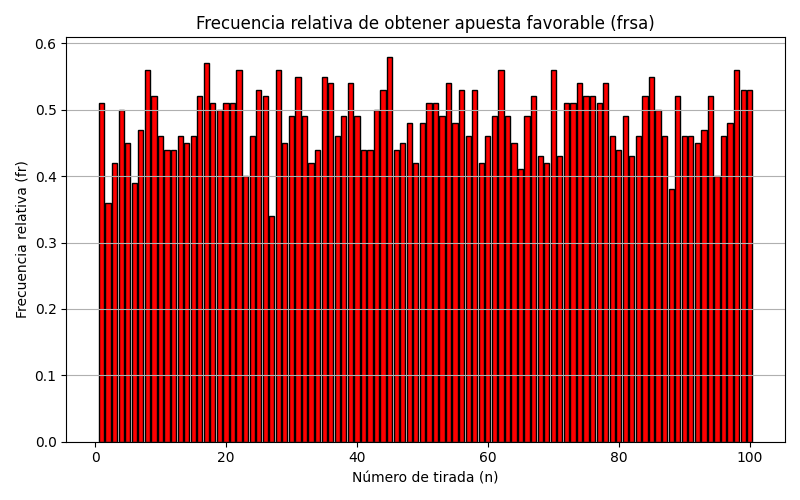
\includegraphics[width=0.48\textwidth]{./Graficas/Frecuencia relativa 100c 100t 1000cap m i rojo.png} &
    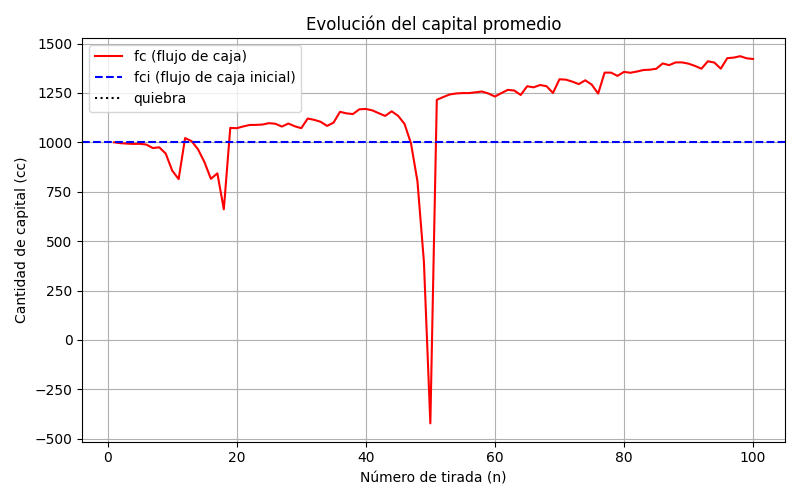
\includegraphics[width=0.48\textwidth]{./Graficas/Promedio 100c 100t 1000cap m i rojo.png}
  \end{tabular}
  \caption{\textbf{Martingala Escenario Ideal} --- Martingala 100 tiradas, 100 corridas, 1000 unidades monetarias, color rojo, capital infinito. Saldo promedio final después de 100 corridas: 1422.20}
\end{figure}

% Figura 2: Martingala Escenario Realista Corto Plazo — 100 cap
\begin{figure}[H]
  \centering
  \begin{tabular}{cc}
    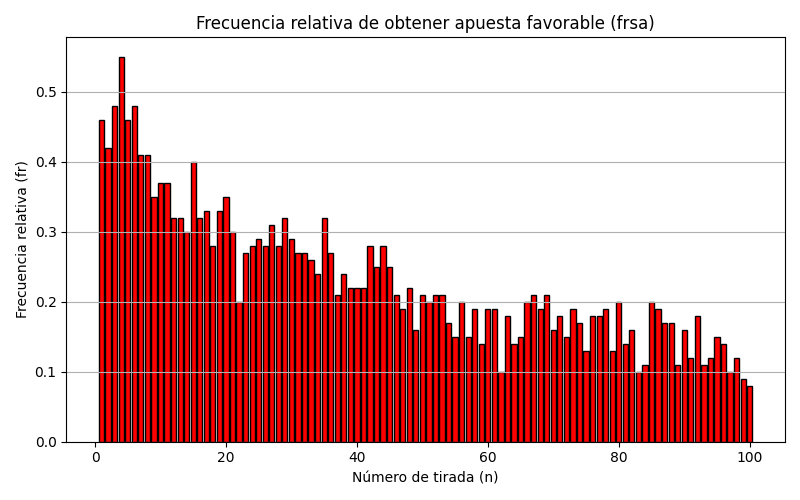
\includegraphics[width=0.48\textwidth]{./Graficas/Frecuencia relativa 100c 100t 100cap f m rojo.png} &
    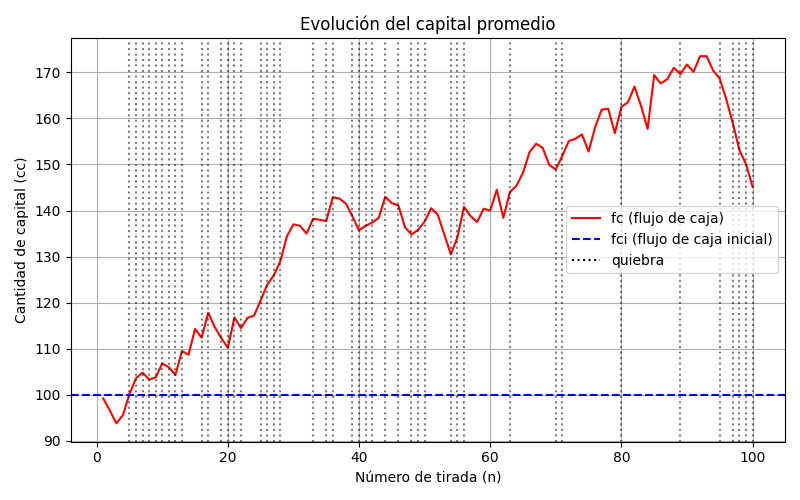
\includegraphics[width=0.48\textwidth]{./Graficas/Promedio 100c 100t 100cap f m rojo.png}
  \end{tabular}
  \caption{\textbf{Martingala Escenario Realista Corto Plazo} --- Martingala 100 tiradas, 100 corridas, 100 unidades monetarias, color rojo, capital finito. Saldo promedio final después de 100 corridas: 87.60. Veces que hubo bancarrota: 74 de 100.}
\end{figure}

% Figura 3: Martingala Escenario Realista Corto Plazo — 1000 cap
\begin{figure}[H]
  \centering
  \begin{tabular}{cc}
    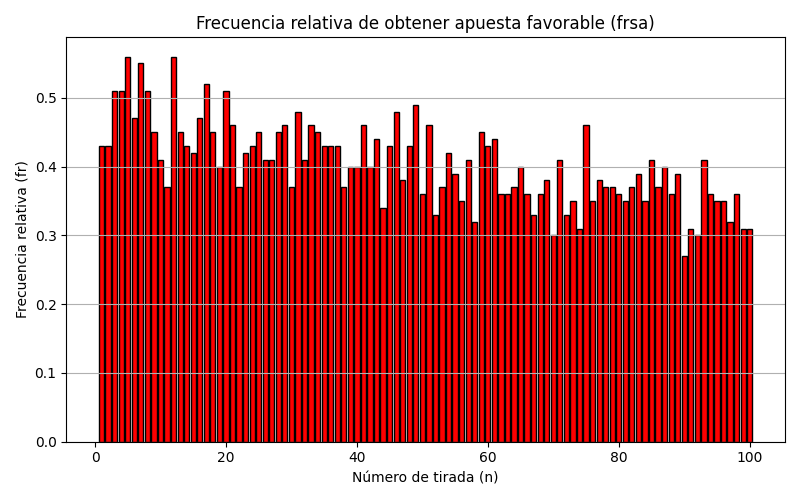
\includegraphics[width=0.48\textwidth]{./Graficas/Frecuencia relativa 100c 100t 1000cap f m.png} &
    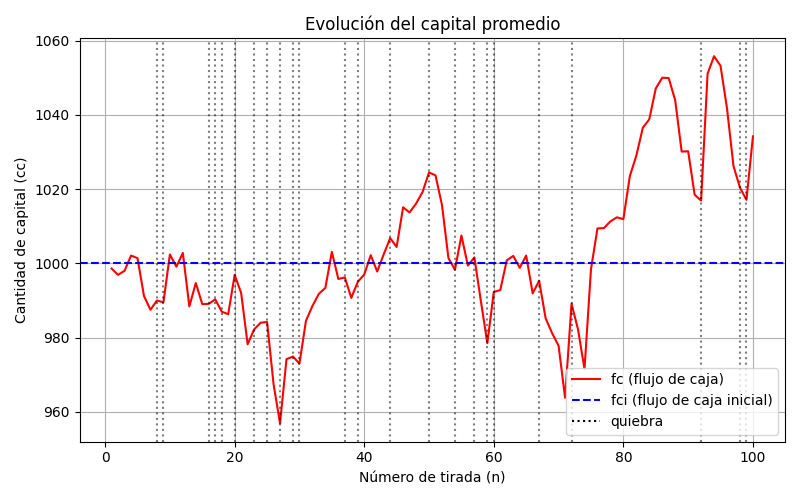
\includegraphics[width=0.48\textwidth]{./Graficas/Promedio 100c 100t 1000cap f m.png}
  \end{tabular}
  \caption{\textbf{Martingala Escenario Realista Corto Plazo} --- Martingala 100 tiradas, 100 corridas, 1000 unidades monetarias, color rojo, capital finito. Saldo promedio final después de 100 corridas: 955.80. Veces que hubo bancarrota: 29 de 100.}
\end{figure}

% Figura 4: Martingala Escenario Realista Corto Plazo — 10000 cap
\begin{figure}[H]
  \centering
  \begin{tabular}{cc}
    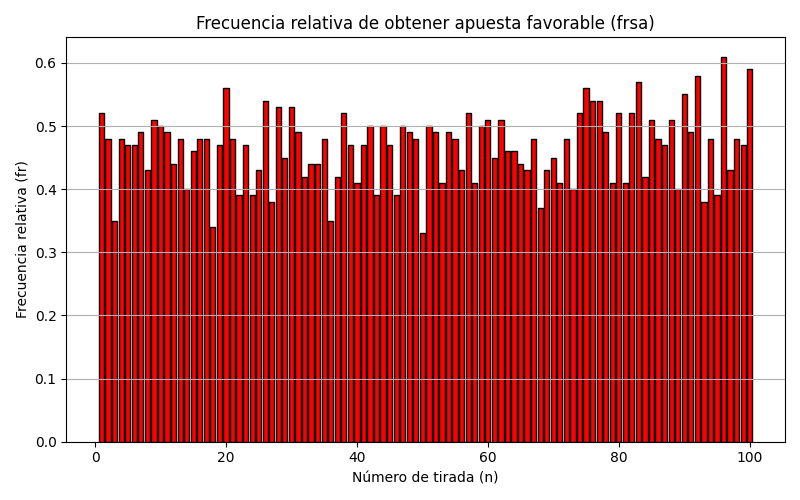
\includegraphics[width=0.48\textwidth]{./Graficas/Frecuencia relativa 100c 100t 10000cap f m rojo.png} &
    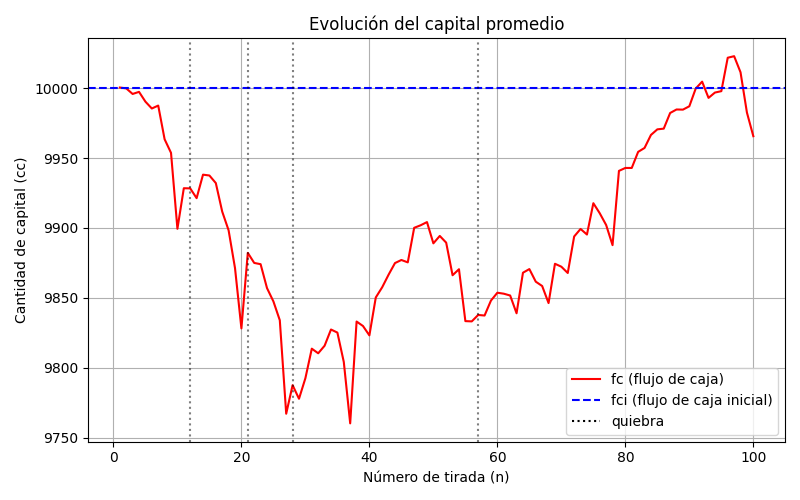
\includegraphics[width=0.48\textwidth]{./Graficas/Promedio 100c 100t 10000cap f m rojo.png}
  \end{tabular}
  \caption{\textbf{Martingala Escenario Realista Corto Plazo} --- Martingala 100 tiradas, 100 corridas, 10000 unidades monetarias, color rojo, capital finito. Saldo promedio final después de 100 corridas: 9960.70. Veces que hubo bancarrota: 4 de 100.}
\end{figure}

% Figura 5: Martingala Escenario Largo Plazo — 1000 cap
\begin{figure}[H]
  \centering
  \begin{tabular}{cc}
    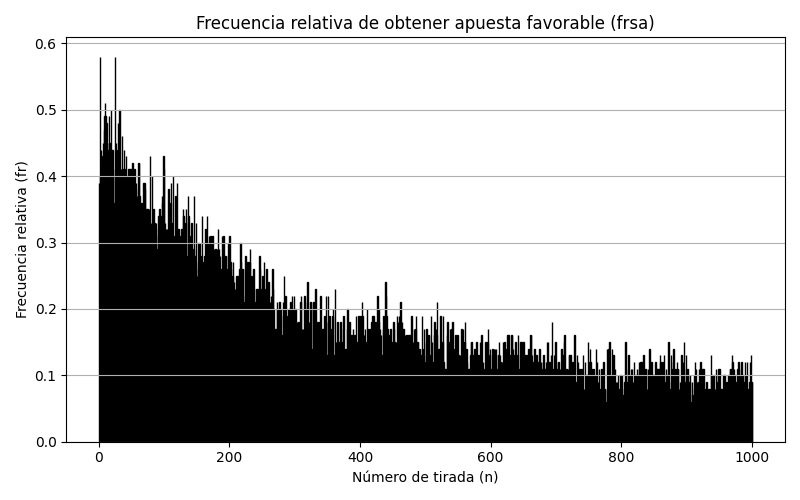
\includegraphics[width=0.48\textwidth]{Graficas/Frecuencia relativa 100c 1000t 1000cap f m rojo.png} &
    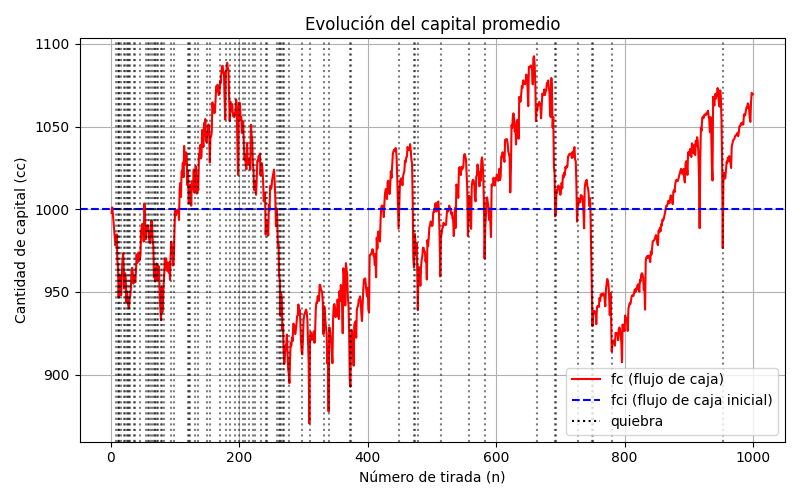
\includegraphics[width=0.48\textwidth]{Graficas/Promedio 100c 1000t 1000cap f m rojo.png}
  \end{tabular}
  \caption{\textbf{Martingala Escenario Largo Plazo} --- Martingala 1000 tiradas, 100 corridas, 1000 unidades monetarias, color rojo, capital finito. Saldo promedio final después de 1000 corridas: 473.40. Veces que hubo bancarrota: 82 de 100}
\end{figure}

% Figura 6: Martingala Numero
\begin{figure}[H]
  \centering
  \begin{tabular}{cc}
    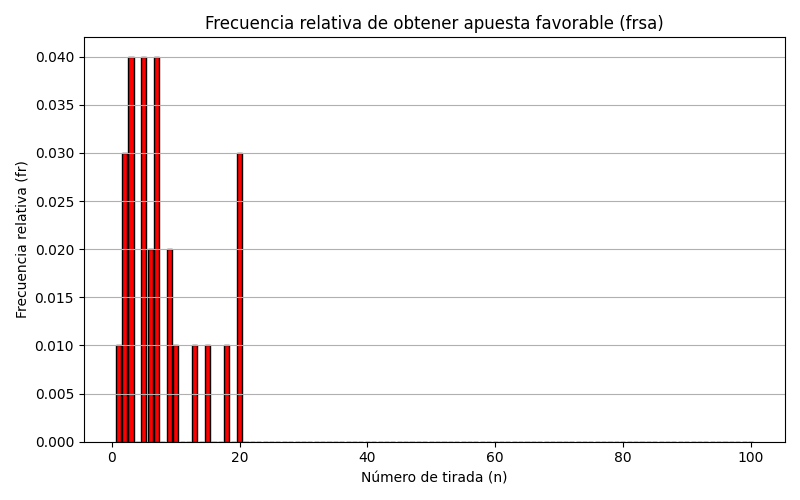
\includegraphics[width=0.48\textwidth]{Graficas/Frecuencia relativa 100c 100t 1000cap f m 1.png} &
    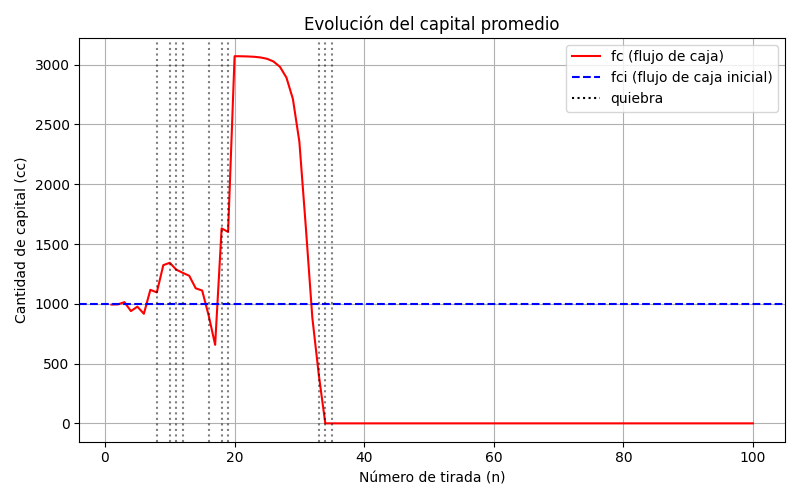
\includegraphics[width=0.48\textwidth]{Graficas/Promedio 100c 100t 1000cap f m 1.png}
  \end{tabular}
  \caption{\textbf{Martingala Apuesta a número} --- Martingala 100 tiradas, 100 corridas, 1000 unidades monetarias, número 1, capital finito. Saldo promedio final después de 100 corridas: 0.00. Veces que hubo bancarrota: 100 de 100}
\end{figure}


\subsection*{Resultados para la estrategia D'Alembert}

% Figura: D'Alembert Escenario Ideal
\begin{figure}[H]
  \centering
  \begin{tabular}{cc}
    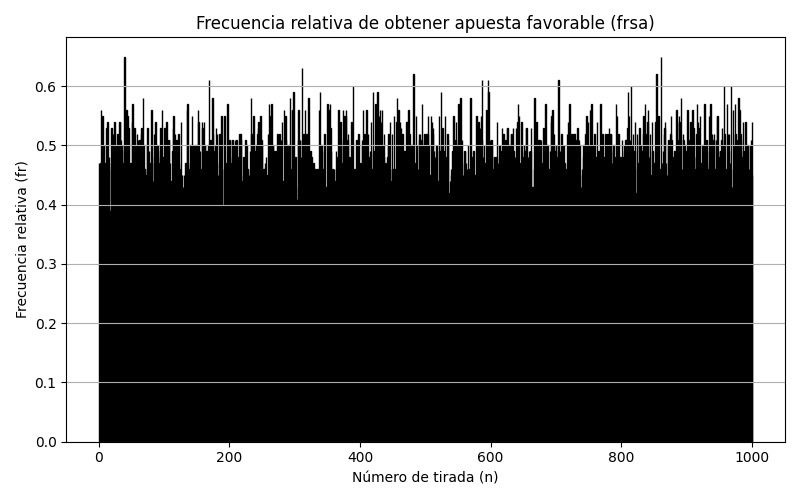
\includegraphics[width=0.48\textwidth]{./Graficas/Frecuencia relativa 100c 1000t 1000cap d i rojo.png} &
    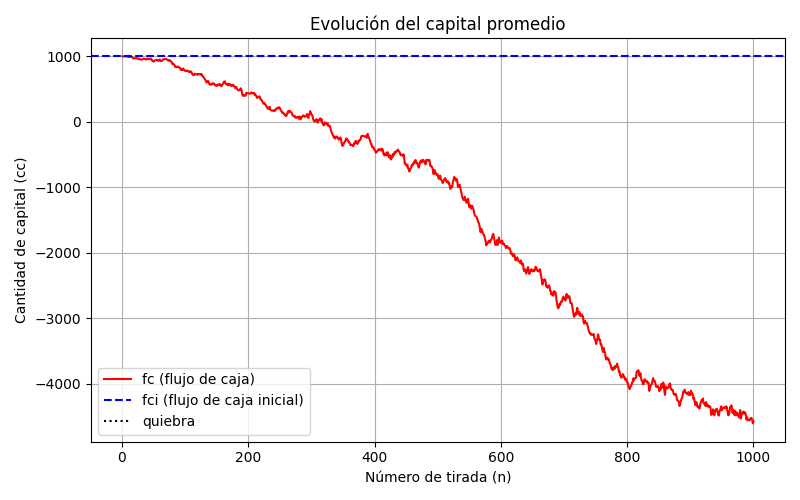
\includegraphics[width=0.48\textwidth]{./Graficas/Promedio 100c 1000t 1000cap d i rojo.png}
  \end{tabular}
  \caption{\textbf{D'Alembert Escenario Ideal} --- D'Alembert 1000 tiradas, 100 corridas, 1000 unidades monetarias, color rojo, capital infinito. Saldo promedio final después de 100 corridas: -5976.00}
\end{figure}


% Figura: D'Alembert Escenario Realista Corto Plazo — 100 cap
\begin{figure}[H]
  \centering
  \begin{tabular}{cc}
    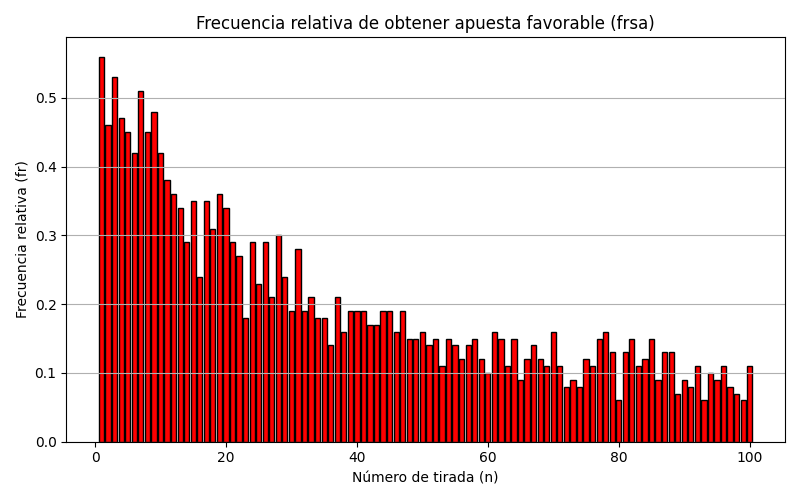
\includegraphics[width=0.48\textwidth]{Graficas/Frecuencia relativa 100c 100t 100cap d f rojo.png} &
    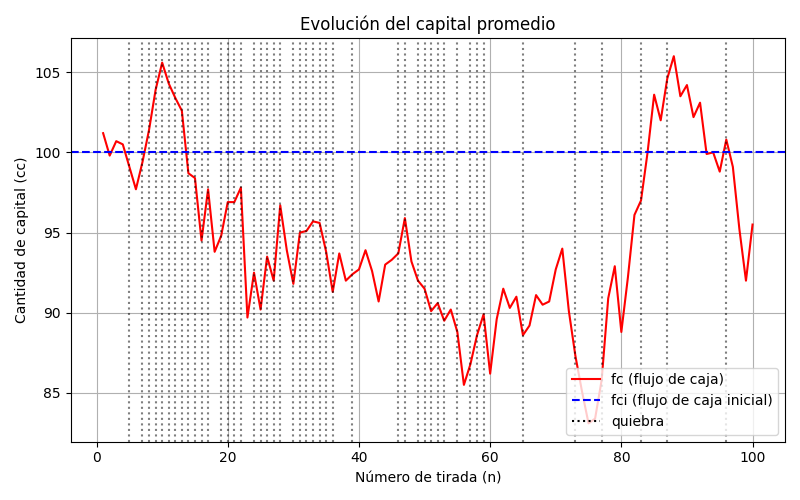
\includegraphics[width=0.48\textwidth]{Graficas/Promedio 100c 100t 100cap d f rojo.png}
  \end{tabular}
  \caption{\textbf{D'Alembert Escenario Realista Corto Plazo} --- D'Alembert 100 tiradas, 100 corridas, 100 unidades monetarias, color rojo, capital finito. Saldo promedio final después de 100 corridas: 74.30. Veces que hubo bancarrota: 81 de 100.}
\end{figure}


% Figura: D'Alembert Escenario Realista Corto Plazo — 1000 cap
\begin{figure}[H]
  \centering
  \begin{tabular}{cc}
    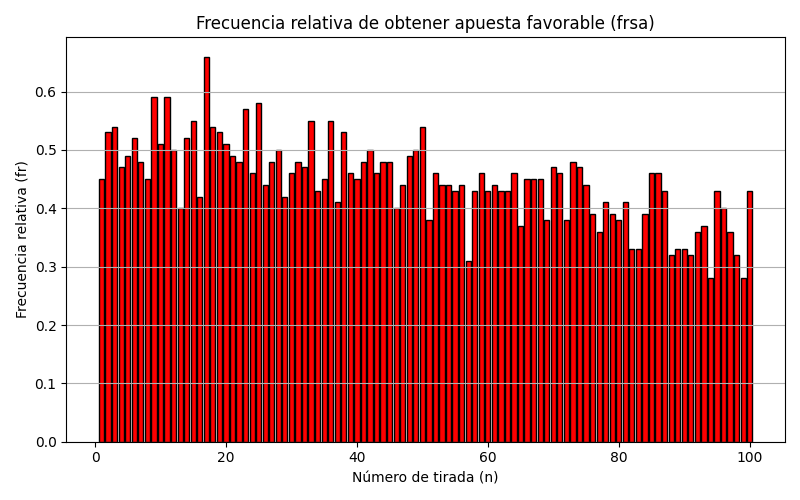
\includegraphics[width=0.48\textwidth]{Graficas/Frecuencia relativa 100c 100t 1000cap d f rojo.png} &
    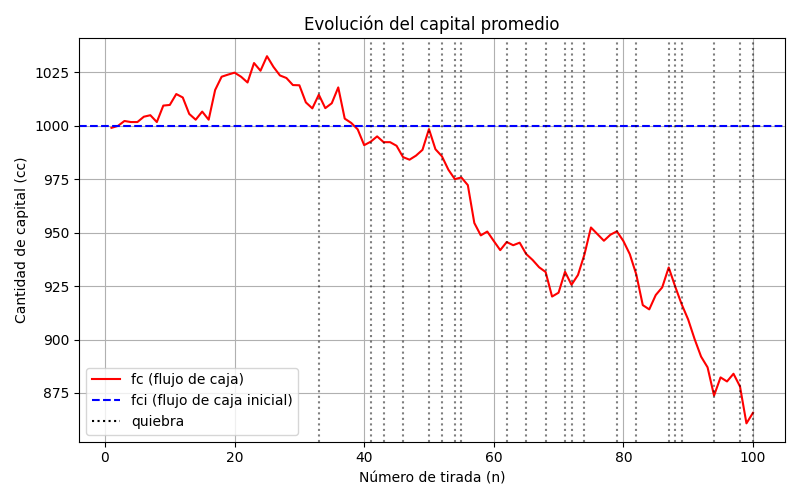
\includegraphics[width=0.48\textwidth]{Graficas/Promedio 100c 100t 1000cap d f rojo.png}
  \end{tabular}
  \caption{\textbf{D'Alembert Escenario Realista Corto Plazo} --- D'Alembert 100 tiradas, 100 corridas, 1000 unidades monetarias, color rojo, capital finito. Saldo promedio final después de 100 corridas: 847.00. Veces que hubo bancarrota: 25 de 100.}
\end{figure}


% Figura: D'Alembert Escenario Realista Corto Plazo — 10000 cap
\begin{figure}[H]
  \centering
  \begin{tabular}{cc}
    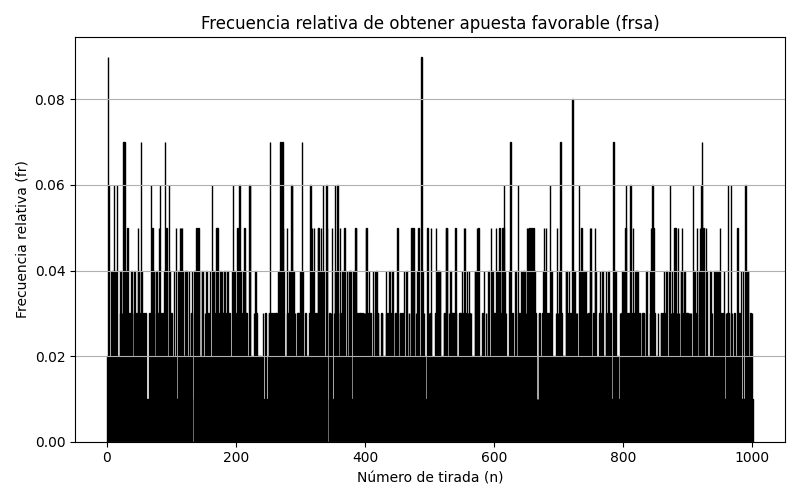
\includegraphics[width=0.48\textwidth]{Graficas/Frecuencia relativa 100c 1000t 1000cap d f rojo.png} &
    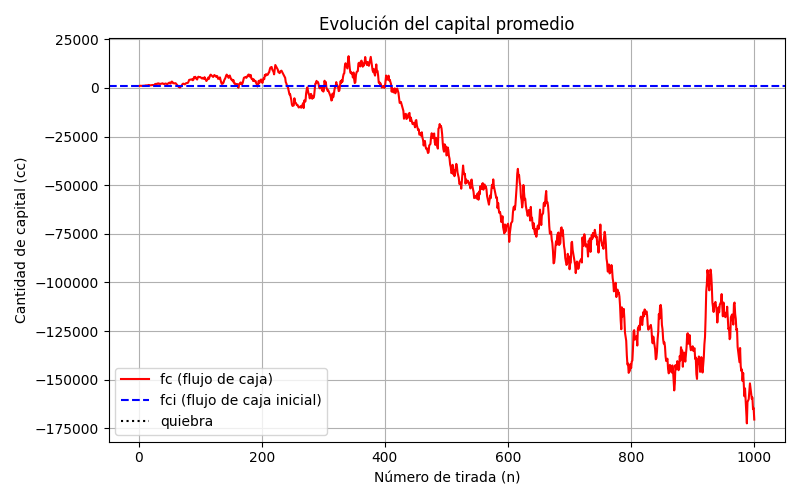
\includegraphics[width=0.48\textwidth]{Graficas/Promedio 100c 1000t 1000cap d f rojo.png}
  \end{tabular}
  \caption{\textbf{D'Alembert Escenario Realista Largo Plazo} --- D'Alembert 100 tiradas, 1000 corridas, 1000 unidades monetarias, color rojo, capital finito. Saldo promedio final después de 100 corridas: 330.00. Veces que hubo bancarrota: 91 de 100.}
\end{figure}

\subsection*{Resultados para la estrategia Fibonacci}

% Figura: Fibonacci Escenario Ideal
\begin{figure}[H]
  \centering
  \begin{tabular}{cc}
    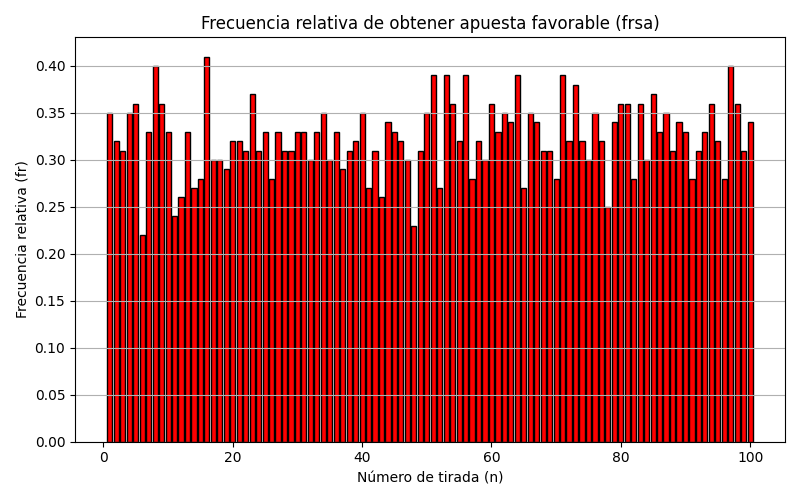
\includegraphics[width=0.48\textwidth]{Graficas/Frecuencia relativa 100c 100t f i docena primera.png} &
    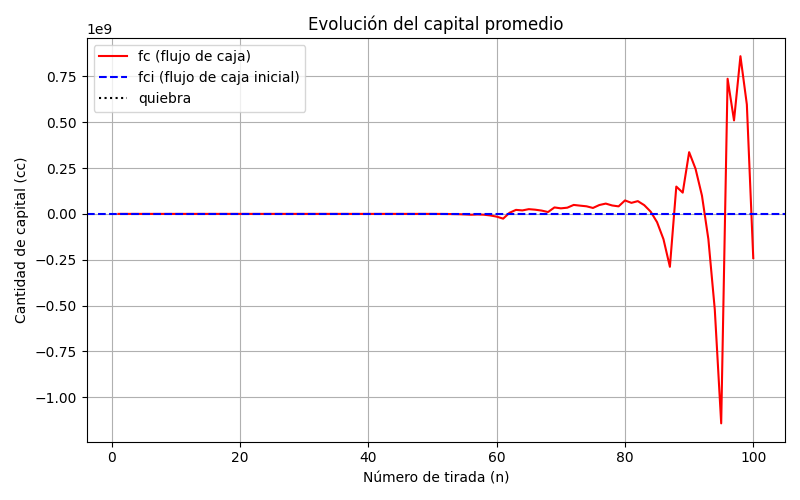
\includegraphics[width=0.48\textwidth]{Graficas/Promedio 100c 100t f i docena primera.png}
  \end{tabular}
  \caption{\textbf{Fibonacci Escenario Ideal} --- Fibonacci 100 tiradas, 100 corridas, 1000 unidades monetarias, primera docena, capital infinito. Saldo promedio final después de 100 corridas: -241016867.60}
\end{figure}

% Figura: Fibonacci Escenario Realista Corto Plazo — 100 cap
\begin{figure}[H]
  \centering
  \begin{tabular}{cc}
    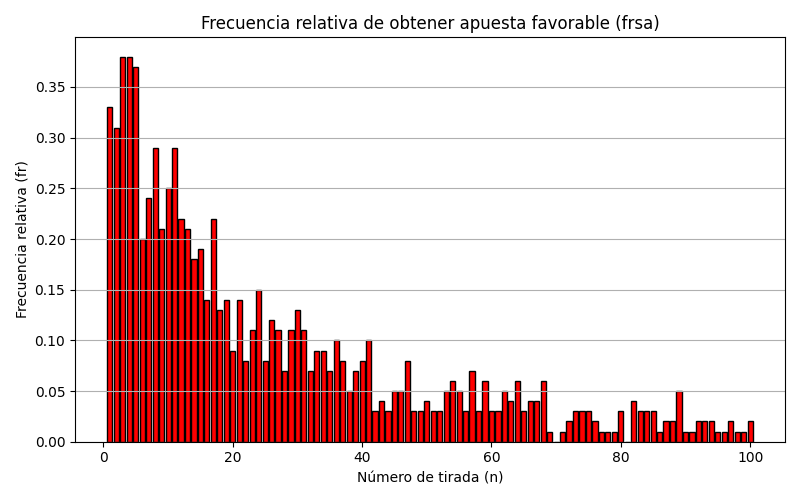
\includegraphics[width=0.48\textwidth]{Graficas/Frecuencia relativa 100c 100t 100cap f docena primera agresivo.png} &
    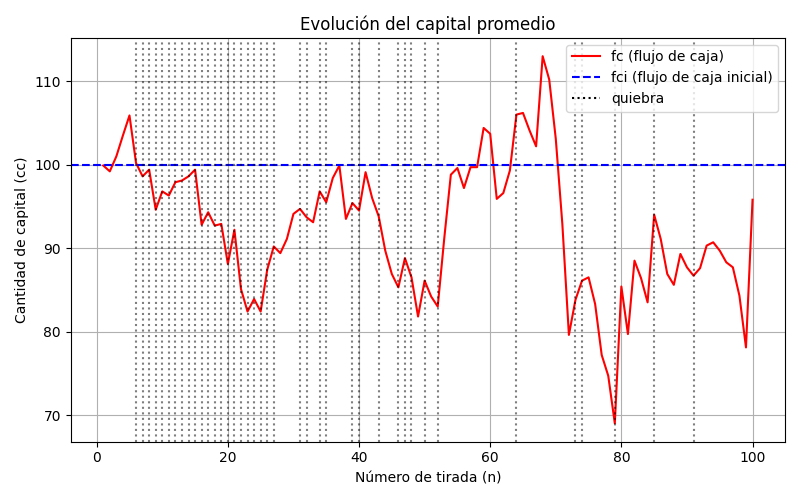
\includegraphics[width=0.48\textwidth]{Graficas/Promedio 100c 100t 100cap f docena primera agresivo.png}
  \end{tabular}
  \caption{\textbf{Fibonacci Escenario Realista Corto Plazo} --- Fibonacci 100 tiradas, 100 corridas, 100 unidades monetarias, primera docena, capital finito. Saldo promedio final después de 100 corridas: 95.80. Veces que hubo bancarrota: 95 de 100.}
\end{figure}

% Figura: Fibonacci Escenario Realista Corto Plazo — 1000 cap
\begin{figure}[H]
  \centering
  \begin{tabular}{cc}
    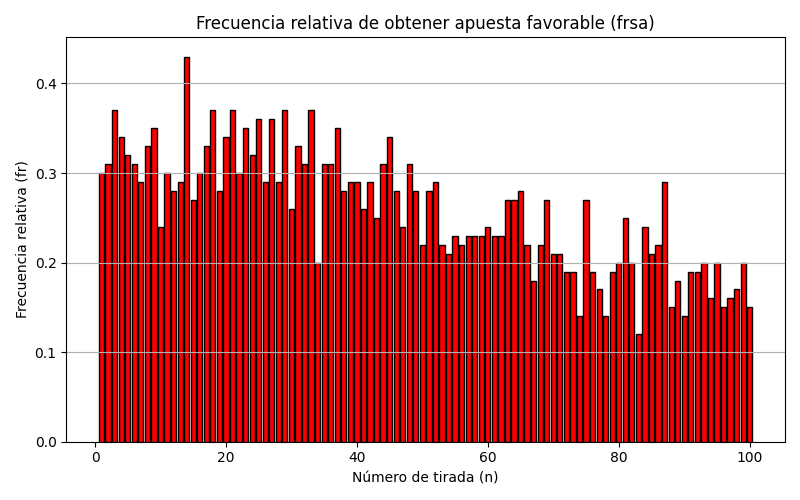
\includegraphics[width=0.48\textwidth]{Graficas/Frecuencia relatival 100c 100t 10000cap f docena primera conservador.png} &
    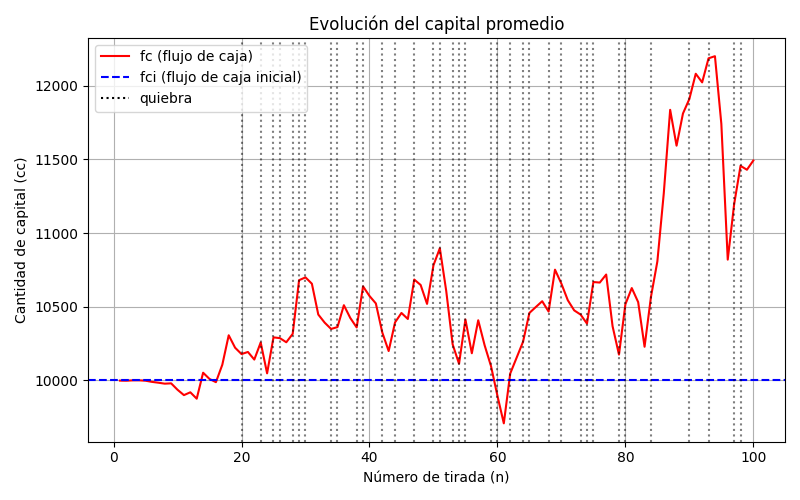
\includegraphics[width=0.48\textwidth]{Graficas/Promedio 100c 100t 10000cap f docena primera conservador.png}
  \end{tabular}
  \caption{\textbf{Fibonacci Escenario Realista Corto Plazo} --- Fibonacci 100 tiradas, 100 corridas, 10000 unidades monetarias, primera docena, capital finito. Saldo promedio final después de 100 corridas: 8327.30. Veces que hubo bancarrota: 49 de 100.}
\end{figure}

% Figura: Fibonacci Escenario Largp Plazo
\begin{figure}[H]
  \centering
  \begin{tabular}{cc}
    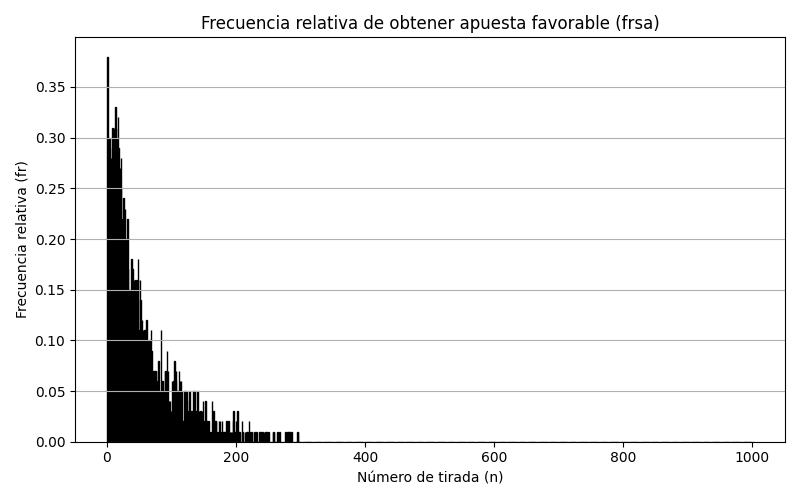
\includegraphics[width=0.48\textwidth]{Graficas/Frecuencia relativa 100c 1000t 1000cap f docena primera largo plazo.png} &
    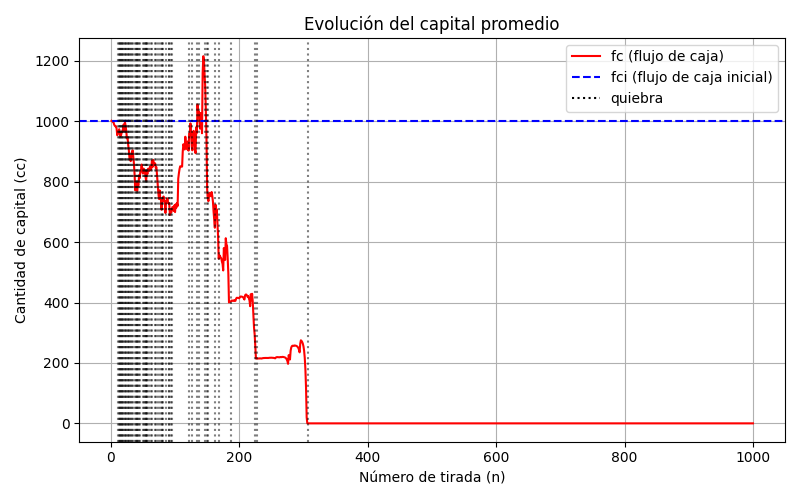
\includegraphics[width=0.48\textwidth]{Graficas/Promedio 100c 1000t 1000cap f docena primera largo plazo.png}
  \end{tabular}
  \caption{\textbf{Fibonacci Escenario Largo Plazo} --- Fibonacci 1000 tiradas, 100 corridas, 1000 unidades monetarias, color rojo, capital finito. Saldo promedio final después de 100 corridas: 0.00. Veces que hubo bancarrota: 100 de 100}
\end{figure}

\subsection*{Resultados para la estrategia Paroli}

% Figura: Paroli Escenario Ideal
\begin{figure}[H]
  \centering
  \begin{tabular}{cc}
    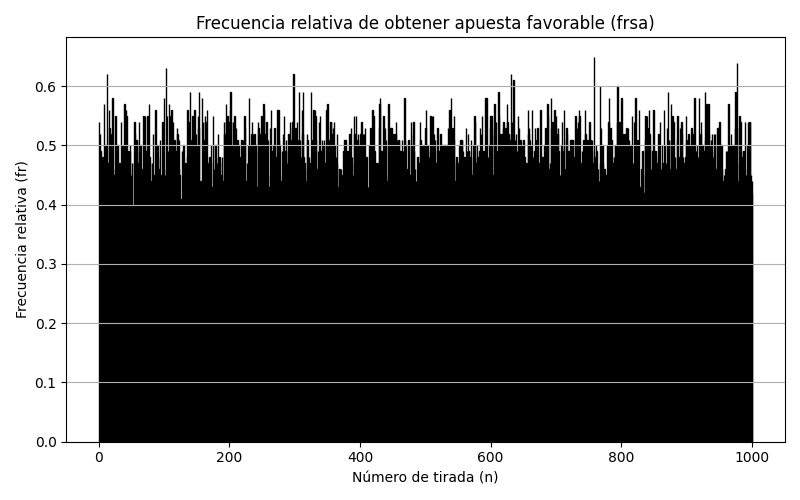
\includegraphics[width=0.48\textwidth]{Graficas/Frecuencia relativa 100c 1000t 1000cap p i rojo.png} &
    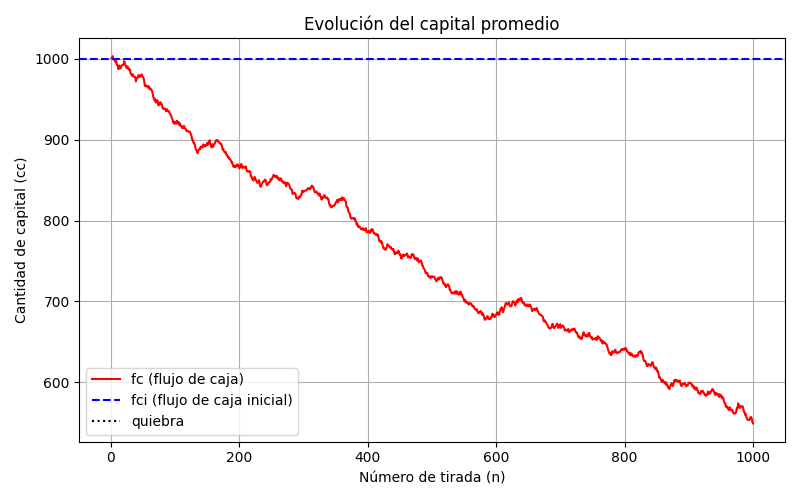
\includegraphics[width=0.48\textwidth]{./Graficas/Promedio 100c 1000t 1000cap p i rojo.png}
  \end{tabular}
  \caption{\textbf{Paroli Escenario Ideal} --- Paroli 1000 tiradas, 100 corridas, 1000 unidades monetarias, color rojo, capital infinito. Saldo promedio final después de 100 corridas: 549.20}
\end{figure}

% Figura: Paroli Escenario Realista Corto Plazo — 100 cap
\begin{figure}[H]
  \centering
  \begin{tabular}{cc}
    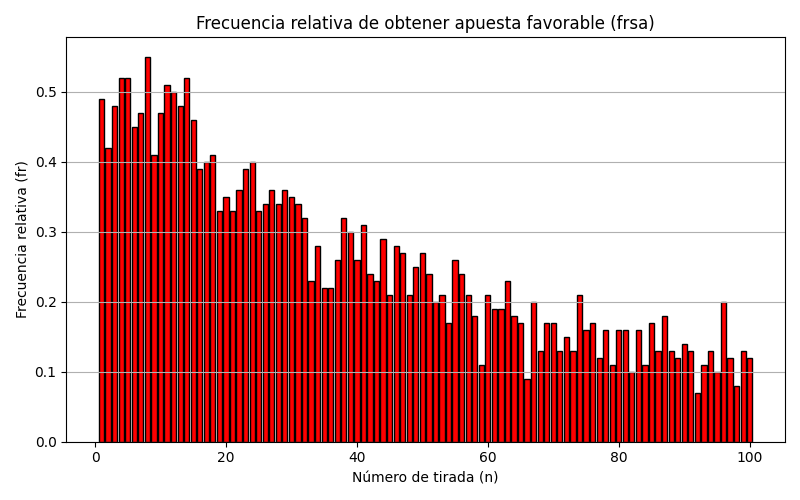
\includegraphics[width=0.48\textwidth]{Graficas/Frecuencia relativa 100c 100t 100cap p f rojo.png} &
    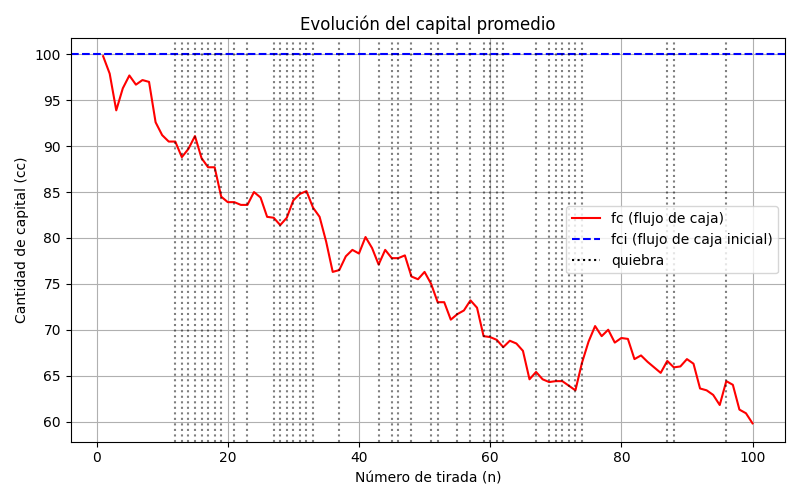
\includegraphics[width=0.48\textwidth]{Graficas/Promedio 100c 100t 100cap p f rojo.png}
  \end{tabular}
  \caption{\textbf{Paroli Escenario Realista Corto Plazo} --- Paroli 100 tiradas, 100 corridas, 100 unidades monetarias, color rojo, capital finito. Saldo promedio final después de 100 corridas: 59.8. Veces que hubo bancarrota: 74 de 100}
\end{figure}

% Figura: Paroli Escenario Realista Corto Plazo — 1000 cap
\begin{figure}[H]
  \centering
  \begin{tabular}{cc}
    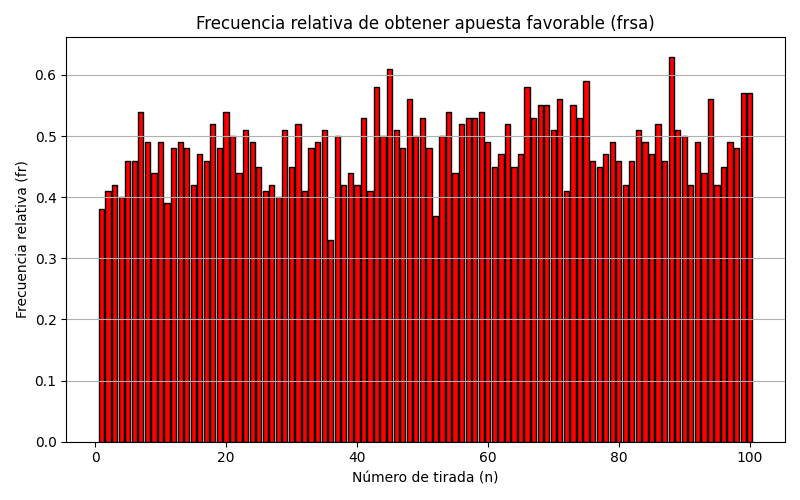
\includegraphics[width=0.48\textwidth]{Graficas/Frecuencia relativa 100c 100t 1000cap p f rojo.png} &
    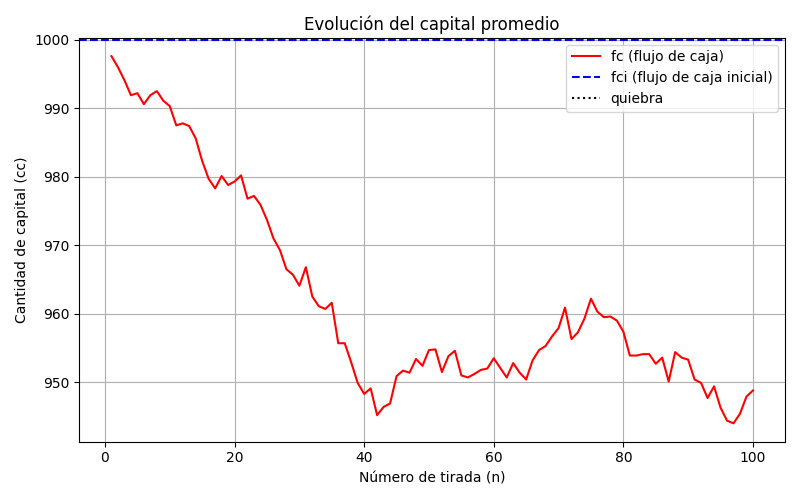
\includegraphics[width=0.48\textwidth]{Graficas/Promedio 100c 100t 1000cap p f rojo.png}
  \end{tabular}
  \caption{\textbf{Paroli Escenario Realista Corto Plazo} --- Paroli 100 tiradas, 100 corridas, 1000 unidades monetarias, color rojo, capital finito. Saldo promedio final después de 100 corridas: 948.80. Veces que hubo bancarrota: 0 de 100}
\end{figure}

% Figura: Paroli Escenario Largo Plazo
\begin{figure}[H]
  \centering
  \begin{tabular}{cc}
    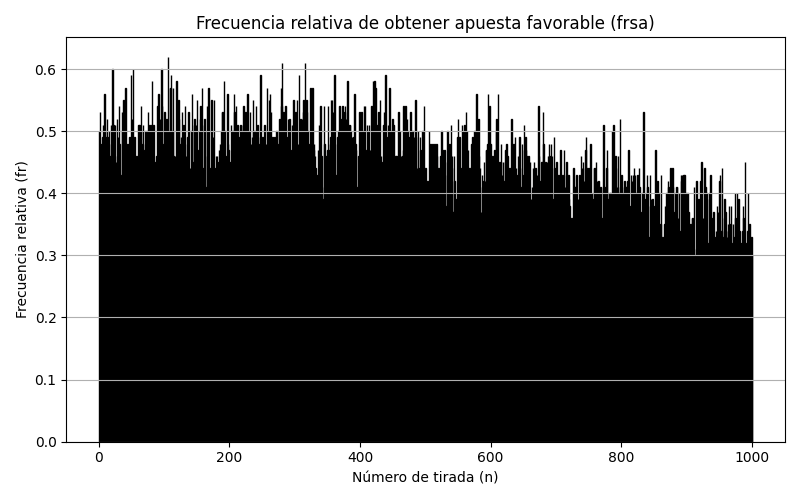
\includegraphics[width=0.48\textwidth]{Graficas/Frecuencia relativa 100c 1000t 1000cap p f rojo.png} &
    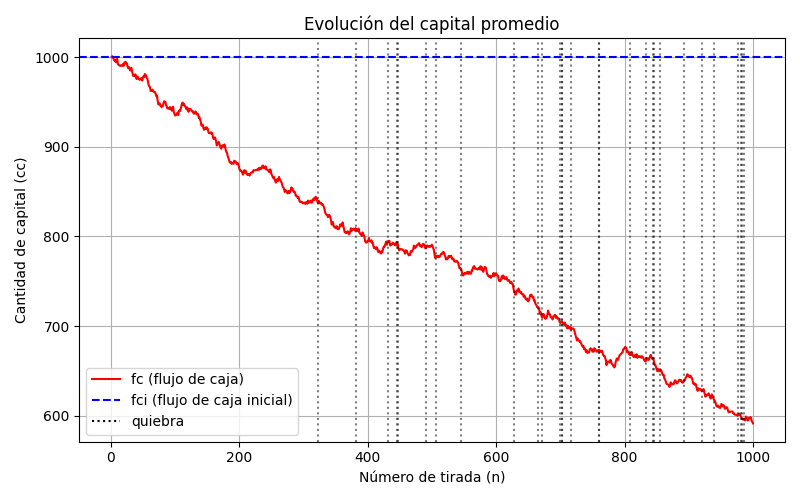
\includegraphics[width=0.48\textwidth]{Graficas/Promedio 100c 1000t 1000cap p f rojo.png}
  \end{tabular}
  \caption{\textbf{Paroli Escenario Largo Plazo} --- Paroli 100 tiradas, 1000 corridas, 1000 unidades monetarias, color rojo, capital finito. Saldo promedio final después de 1000 corridas: 591.50. Veces que hubo bancarrota: 31 de 100}
\end{figure}

\section{Discusión}

El análisis de sensibilidad estructurado a través de los tres bloques experimentales permite demostrar de forma empírica que, independientemente de la progresión matemática utilizada, ninguna estrategia es capaz de alterar la ventaja intrínseca de la casa ($1 - P(\text{Color}) - P(\text{Cero}) \approx 51.35\%$), evidenciando dinámicas de riesgo marcadamente distintas.

\subsection{Estrategia Martingala}
    La estrategia Martingala exhibió el comportamiento más contrastante del estudio. En el escenario de capital infinito (Bloque 1), cumplió con la hipótesis de recuperación teórica logrando un saldo promedio final de $1422.20$ u.m. No obstante, al introducir la restricción de capital finito (Bloque 2), la progresión geométrica se convirtió en un mecanismo de quiebra exponencial:
\begin{itemize}
    \item \textbf{Enfoque Agresivo ($f = 0.1$, $C_0 = 100$):} El margen de amortiguación es prácticamente nulo. Una racha de solo 4 pérdidas consecutivas deriva en bancarrota, resultando en una tasa de quiebra del 74\% y un saldo promedio de $87.60$ u.m.
    \item \textbf{Enfoque Moderado ($f = 0.01$, $C_0 = 1000$):} Aumentar el capital mitiga parcialmente el riesgo en el corto plazo (29\% de quiebras), finalizando con $955.80$ u.m.
    \item \textbf{Enfoque Conservador ($f = 0.001$, $C_0 = 10000$):} Ofrece la mayor resiliencia a corto plazo, reduciendo la bancarrota a solo 4 de 100 corridas ($9960.70$ u.m. de saldo promedio).
\end{itemize}
Sin embargo, al pasar al largo plazo (Bloque 3), la Martingala colapsa de forma inevitable a pesar de contar con una fracción moderada ($f = 0.01$): la tasa de bancarrota se dispara al 82\% con un saldo remanente de solo $473.40$ u.m. 

En el caso de la Martingala a Número Único ($p \approx 0.027$), la simulación arrojó una tasa de destrucción absoluta (100\% de quiebras, saldo $0.00$ u.m.). Esto ocurre porque la velocidad de la progresión geométrica es infinitamente superior a la frecuencia de acierto, demostrando la incompatibilidad de esta estrategia en apuestas complejas.

\subsection{Estrategia D'Alembert}
La estrategia D'Alembert demostró ser más longeva que la Martingala ante capitales acotados debido a su progresión aritmética. En el corto plazo con $C_0 = 1000$ y $f=0.01$, la tasa de quiebra se mantuvo en un aceptable 25\% (saldo promedio de $847.00$ u.m.). 

Sin embargo, el experimento arrojó una anomalía teórica en el escenario de capital infinito: el saldo promedio final se desplomó drásticamente a $-5976.00$ u.m. Este fenómeno ocurre porque, al no existir la condición de parada por quiebra, la simulación permite que la progresión de apuestas crezca linealmente durante las rachas negativas. Como la probabilidad de ganar en apuestas sencillas es menor al 50\% ($48.65\%$), el jugador acumula estadísticamente más pérdidas que ganancias. Al ser una progresión lenta, el sistema no logra "recuperar de un solo golpe" como la Martingala, sino que arrastra un arrastre negativo acumulativo que, en el largo plazo (Bloque 3, capital finito), se traduce en un 91\% de bancarrotas y un saldo remanente de $330.00$ u.m.

\subsection{Estrategia Fibonacci}
La progresión basada en la sucesión de Fibonacci se ejecutó sobre apuestas a Docena ($p \approx 0.324$). Los resultados fueron catastróficos, desmitificando la supuesta "suavidad" de esta estrategia.

En el escenario de capital infinito, el saldo promedio arrojó una pérdida astronómica de $-241,016,867.60$ u.m. Al apostar a una docena, el jugador pierde el $67.57\%$ de las veces. Esto genera rachas de pérdidas consecutivas extremadamente largas que fuerzan a la sucesión de Fibonacci a escalar hacia números elevados. A diferencia de la Martingala que recupera todo con un acierto, el multiplicador $2:1$ de la docena bajo el sistema Fibonacci solo permite retroceder dos posiciones en la serie por cada victoria. Si las victorias no se encadenan rápidamente, el valor de la apuesta se vuelve insostenible. 

Esto se reflejó directamente en el escenario de capital finito: bajo el enfoque agresivo ($C_0 = 100$), la tasa de quiebra fue del 95\%. Incluso bajo el enfoque conservador ($C_0 = 10000$), ocurrió un 49\% de bancarrotas. En el largo plazo (Bloque 3), la convergencia hacia la ruina fue absoluta (100\% de quiebras, saldo promedio $0.00$ u.m.), demostrando que es la estrategia menos eficiente y más destructiva del estudio cuando se asocia a probabilidades mucho menores a $0.5$.

\subsection{Estrategia Paroli}
El Paroli presentó una dinámica matemática opuesta a las tres anteriores. En lugar de arriesgar más capital propio durante las pérdidas, el sistema incrementa la apuesta únicamente utilizando las ganancias de una racha activa. 

Los datos empíricos validan esta premisa de seguridad:
\begin{itemize}
    \item \textbf{Capital Infinito / Largo Plazo:} Finalizó con un saldo positivo de $549.20$ u.m. tras 1000 tiradas.
    \item \textbf{Corto Plazo Moderado ($C_0 = 1000$):} Registró un extraordinario \textbf{0\% de quiebras}, finalizando con un promedio de $948.80$ u.m. 
    \item \textbf{Largo Plazo ($n = 1000$, $C_0 = 1000$):} Sostuvo la menor tasa de bancarrota de todo el estudio para pruebas extensas, con solo un 31\% de quiebras y un saldo remanente positivo de $591.50$ u.m.
\end{itemize}
El punto débil del Paroli se evidenció en el enfoque agresivo ($C_0 = 100$), donde la tasa de quiebra fue del 74\% con un saldo final de $59.80$ u.m. Esto demuestra que, aunque el sistema protege la bancarrota al resetear a la apuesta base tras una pérdida, si el flujo de caja inicial es extremadamente bajo ($f=0.1$), las pérdidas gotean de forma constante de la apuesta base antes de que el jugador logre encadenar la racha de victorias sucesivas necesaria para generar un pico de ganancia. El Paroli no vence matemáticamente a la casa, pero estadísticamente es el único sistema que demostró una gestión de riesgo favorable para el jugador.

\section{Conclusión}

La conclusión matemática y real es una sola: La casa siempre gana y no existe ninguna estrategia que pueda cambiar eso. Ningún sistema de apuestas, por más inteligente que parezca en los papeles, logra modificar las probabilidades de la ruleta. El casillero verde del cero ($0$) está ahí para asegurar que, tarde o temprano, el casino se quede con una ventaja a su favor.

Gracias a los tres bloques de pruebas que armamos, pudimos rescatar las siguientes verdades sobre cada estrategia:

\begin{itemize}
    \item \textbf{La Martingala es una trampa a largo plazo:} En el escenario "ideal" sin límite de capital parece perfecta (terminó con ganancia de $1422.20$ u.m.), pero en la vida real es peligrosa. Presentarse con poco capital ($100$ u.m.), significa exponerse a que una mala racha de 4 o 5 tiradas derive en bancarrota (74\% de quiebras). Peor aún si se apuesta a un número único: La probabilidad de bancarrota es de el 100\% de las veces porque la apuesta sube mucho más rápido de lo que se demora en adivinar un número.
    
    \item \textbf{D'Alembert resiste pero no recupera:} Al subir y bajar las apuestas de a una unidad (una progresión lenta), protege más el bolsillo en el corto plazo. El problema es que al entrar en una racha perdedora, lleva a una pérdida tan pesada que es prácticamente imposible recuperarse. Por eso en capital infinito dio una pérdida ridícula de $-5976.00$ u.m. y a largo plazo derivó en bancarrota el 91\% de las veces.
    
    \item \textbf{Fibonacci a la docena es destructiva:} Al aplicarse a las docenas (donde se pierde el 67\% de las veces), las malas rachas son largas. Como la estrategia hace retroceder solo dos casilleros cuando se gana, nunca se terminan de tapar los agujeros de las pérdidas anteriores. ¿El resultado? Dio pérdidas millonarias en capital infinito y 100\% de quiebras a largo plazo. 
    
    \item \textbf{Paroli es la única estrategia que protege el bolsillo:} Fue, por lejos, la estrategia menos riesgosa. Al ser una progresión positiva (solo se apuesta fuerte al entrar en una racha positiva con capital del casino), se protege el capital propio. En las pruebas de corto plazo tuvo un 0\% de quiebras y a largo plazo fue la que más sobrevivió (solo 31\% de quiebras). No vence a la ruleta, pero es la única que asegura no llegar a la bancarrota rápidamente.
\end{itemize}

En resumen, la simulación por computadora nos permitió demostrar de forma objetiva que los sistemas "infalibles" de apuestas son un mito. La ruleta europea está diseñada para que el jugador pierda dinero a la larga. Por ende, estas estrategias jamás deben pensarse como un método financiero para ganar dinero.

\section{Referencias}
\begin{itemize}
  \item Sportium Blog: “3 simples estrategias para ganar en la ruleta que cualquiera puede intentar”, \url{https://blog.sportium.es/3-simples-estrategias-para-ganar-en-la-ruleta-que-cualquiera-puede-intentar/}
  \item R. López Briega, “Probabilidad y estadística con Python”, \url{https://relopezbriega.github.io/blog/2015/06/27/probabilidad-y-estadistica-con-python/}
  \item Matplotlib Documentation, “Users Guide”, \url{https://matplotlib.org/stable/users/index.html}
  \item NumPy Documentation, “User Guide”, \url{https://numpy.org/doc/stable/user/}
  \item Python Standard Library, “random — Generators of random numbers”, \url{https://docs.python.org/3/library/random.html}
  \item Wikipedia, “Ruleta”, \url{https://es.wikipedia.org/wiki/Ruleta}
  \item Wikipedia, “Martingala”, \url{https://es.wikipedia.org/wiki/Martingala}
  \item Wikipedia, “D'Alembert”, \url{https://es.wikipedia.org/wiki/Principio_de_d%27Alembert}
  \item Wikipedia, “Fibonacci”, \url{https://es.wikipedia.org/wiki/Sucesión_de_Fibonacci}
  \item Pokerstars, “Paroli”, \href{https://www.pokerstars.es/casino/news/los-grandes-sistemas-de-la-ruleta-el-sistema-paroli/}{pokerstars.es/.../el-sistema-paroli/}
\end{itemize}

\end{document}

